\chapter{AsthmAPP}
\label{chp:description}

This chapter gives a description of AsthmAPP, through textual description and screenshots. Please note that the main language of the application is Norwegian. We have translated the text where it seemed appropriate. 

\section{Architecture and Technology}

\subsection{System Architecture}
\label{sec:architecture}
Figure \ref{fig:basic-architecture} shows an overview of the architecture we used for our products (\ab{} included). We reused some of the components Aaberg et. al. created during Customer Driven Project\cite{CustomerDriven}. 

Data is stored at a MySQL database hosted by NTNU. \app{} and \ab{} accessed the database through a PHP-server, which is also hosted by NTNU. The reason for accessing the database through a PHP-server is twofold. First, it is difficult to access the database when a device is not located on the local network at NTNU. It would be required that a user had VPN installed to access the NTNU network at their smartphones, which is not ideal from a performance point-of-view.

Second, by having a webservice that interprets the results given by the database, it becomes easier for the client to deserialize these results, as they are given as JSON-objects\footnote{JavaScript Object Notation}.    

When one of the applications want to store data to the database, they do a HTTP POST, with the data as POST parameters, to a predefined route on the webservice. When the application wants to retrieve data from the database, it does a HTTP GET to the webservice, which extracts the data requested from the database, formats it to JSON, and returns the data to the application.  

By having a webservice layer between the applications and the database, the system scalability suffers, but modifiability is increased, which we considered as a good trade-off at the current state of our project. 

\begin{figure}
		\centering
			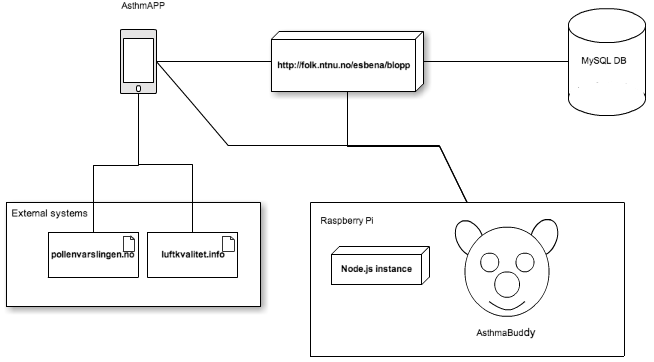
\includegraphics[width=0.60\paperwidth]{Pictures/system-architecture.png}
		\caption{System Architecture}
		\label{fig:basic-architecture}
\end{figure}

\subsection{Technology and Frameworks Used in AsthmAPP}
\label{sec:techandframeinapp}
\app{} is developed in native Android code, which implies using Java as the programming language and the Android Application Framework\fnurl{Android Application Framework}{http://developer.android.com/develop/index.html}. Additionally, we used the following frameworks to ease the development: 

\paragraph{Gson} As mentioned in previously, our webservice gives out JSON-formatted objects of data stored in our database. We used Google's Gson-library\fnurl{Google Gson}{https://code.google.com/p/google-gson/} to deserialize these objects into Java objects.

\paragraph{JodaTime} Java's default implementation of time is cumbersome to work with, with a lot of it's functionality deprecated. JodaTime\fnurl{JodaTime}{http://www.joda.org/joda-time/} is an open source project that seeks to handle time in a proper manner on the Java platform.     


\section{How Usability Research has Affected our Design}
\label{sec:usability-affect-design}
While designing AsthmAPP, we strived for an easy-to-use design with a good overview, in addition to the Android Design Principles\cite{androiddesign}. We have also taken Shneidermann's eight golden rules into consideration when designing \app{}\cite{shneiderman2003designing}. 
We tried to lighten the short-term memory load by using a combination of sounds, pictures and text to tell the user the options that are available or what is expected from the user. During a treatment the user is prompted to take action in order to continue through the process, giving the user a locus of control. 
The layout for both partitions of AsthmAPP gives a general overview, and has few shortcuts between the different elements. To navigate from one element to another the user will have to go via the main menu. While this breaks with Shneidermann's rules and the Android design principles, we believed that the solution we found is the preferrable one.


\section{Child partition}
\label{sec:description-child-partition}
The child partition of our application consists mainly out of four parts. When Aaberg et. al. created the original application, they wanted a conceptual look and feel throughout the applications. They used images of Karotz in the application in order to introduce a sense of completeness, i.e. the Karotz bound CAPP, GAPP and KAPP together. 

\subsection{Treatment}
\label{sec:sec:description-treatment}
Figure \ref{fig:capp_start_treatment} shows a screenshot for the application when the child starts his/her treatment. This sequence may be started by on of two events: (i) \emph{The child reacts to an alarm set in the parent partition}, or (ii) \emph{The child needs to take his/her medicine by need}. If (ii) is the case, the child is instructed to pick the medicine from a list shown by the application. If (i) is the case, the medicine is chosen beforehand. When a child has started his/her treatment, he/she is taken through an animated sequence, which reacts when a child interacts with the device. In addition, the child is being told what to do by the comforting voice of Andreas Ystmark\footnote{A classmate of ours at NTNU}.  


\subsection{Showing rewards}
\label{sec:description-show-rewards}
Figure \ref{fig:capp_stars} shows a screenshot for the application when the child wants to review how many stars he/she has received, based on the amount of treatments completed. We have made two design decisions for our reward system. Firstly, we do not want stars to be removed. We do not want the child to feel that credits are being removed from him/her. Secondly, we cannot assume that children are able to read, and thus we have made the stars countable, and hopefully the child is able to comprehend how many stars he/she actually has. In addition, we provide some help to those who are able to read numbers, by showing the number of stars a child has on the top of the screen.      

\subsection{Shop}
\label{sec:description-shop}
In the shop, children are allowed to select rewards given by their parent(s). Figure \ref{fig:child-possible-rewards} and \ref{fig:child-bought-rewards} show an inside-view of our shop. Children can buy a reward by pressing the selected reward in the menu. Due to time constraints and lack of good software solutions, we have not been able to implement a voice over, so the children may need help with reading the names of the rewards. The possibility of adding pictures to represent the reward should make it easier for the children. 


\subsection{Treatment instructions}
\label{sec:description-instructions}
The treatment instructions is a book-styled instruction set which shows generically how to take the medicine. 
The following steps are included in the instructions: 
\begin{enumerate}
  \item Shake the inhaler to loosen the particles. 
  \item Take the cap of the inhaler.
  \item Attach the inhaler to the inhaling chamber.
  \item Cover nose and mouth with the inhaling chamber.
  \item Press the inhaler until you hear a sound.
  \item Let the child breathe calmly in and out 10 times.
  \item Let the child wash his/her mouth.
\end{enumerate} 

\begin{figure}
	\begin{minipage}[t]{0.3\linewidth}
		\centering
			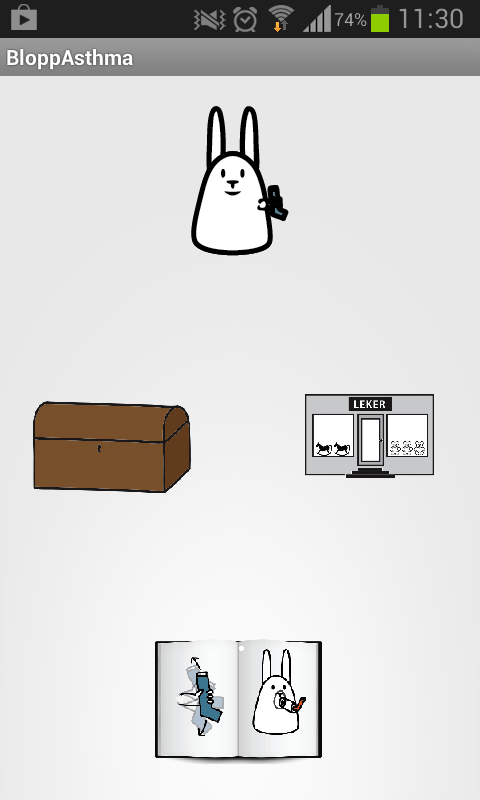
\includegraphics[width=0.20\paperwidth]{Pictures/new-screenshots/kid-menu.png}
		\caption{Main menu of child partition}
		\label{fig:child-menu}
	\end{minipage}
	\hspace{0.5cm}
	\begin{minipage}[t]{0.3\linewidth}
		\centering
			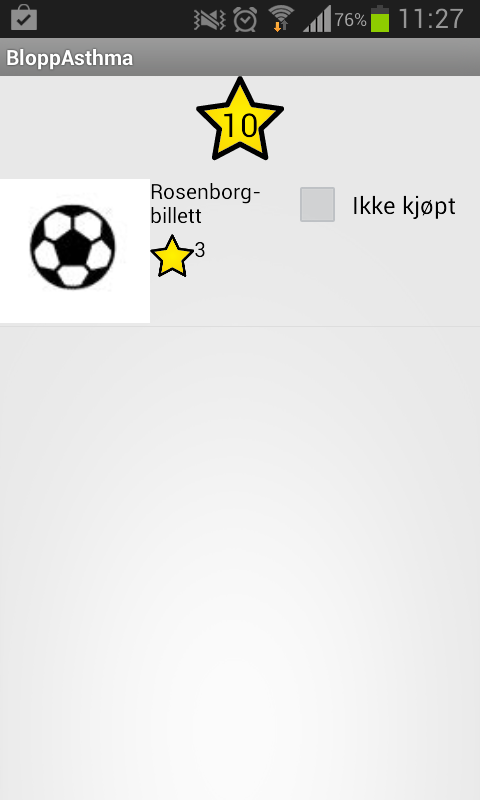
\includegraphics[width=0.20\paperwidth]{Pictures/new-screenshots/child-possible-rewards.png}
		\caption{Possible rewards a child can choose from}
		\label{fig:child-possible-rewards}
	\end{minipage}
	\hspace{0.5cm}
	\begin{minipage}[t]{0.3\linewidth}
		\centering
			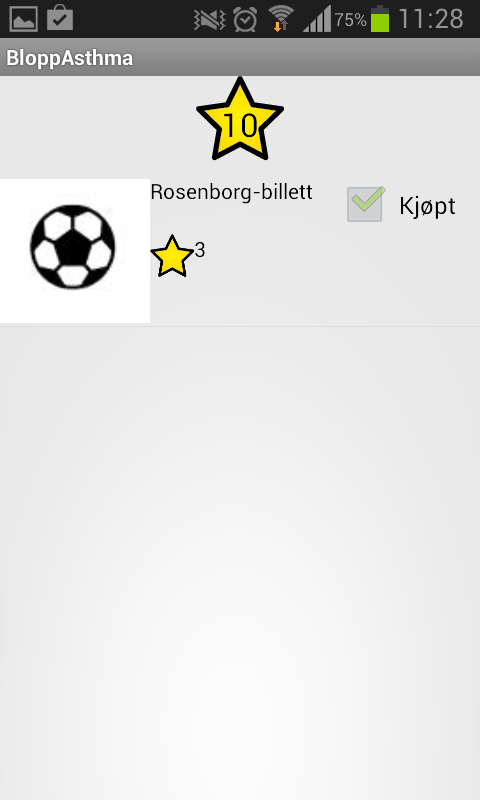
\includegraphics[width=0.20\paperwidth]{Pictures/new-screenshots/child-bought-reward.png}
		\caption{A child has bought the reward}
		\label{fig:child-bought-rewards}
	\end{minipage}
\end{figure}

\begin{figure}
	\begin{minipage}[t]{0.4\linewidth}
		\centering
			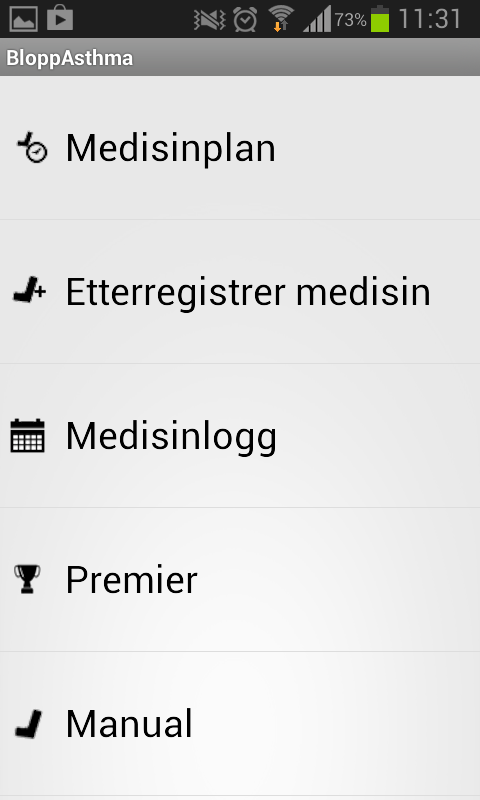
\includegraphics[width=0.20\paperwidth]{Pictures/new-screenshots/parent-menu.png}
		\caption{Main menu of partent partition}
		\label{fig:parent_main_menu}
	\end{minipage}
	\hspace{3cm}
	\begin{minipage}[t]{0.4\linewidth}
		\centering
			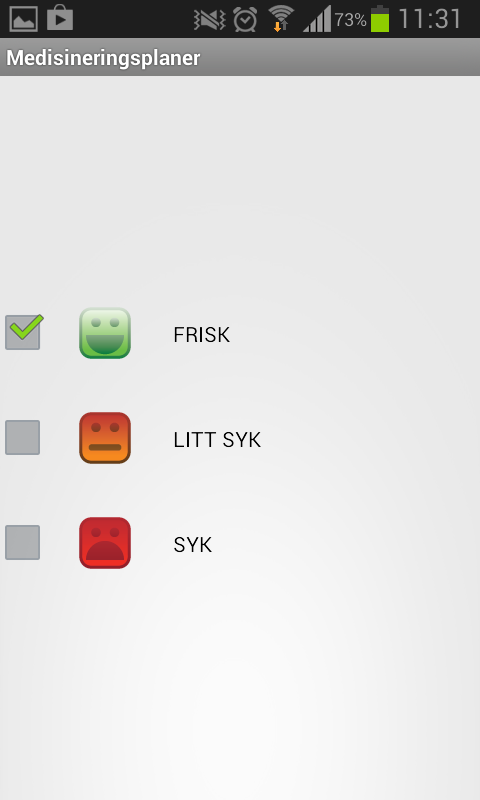
\includegraphics[width=0.20\paperwidth]{Pictures/new-screenshots/medicine-plans.png}
		\caption{Available medicine plans}
		\label{fig:parent_medicine_plans}
	\end{minipage}
	%NEW LINE
	\begin{minipage}[t]{0.4\linewidth}
		\centering
			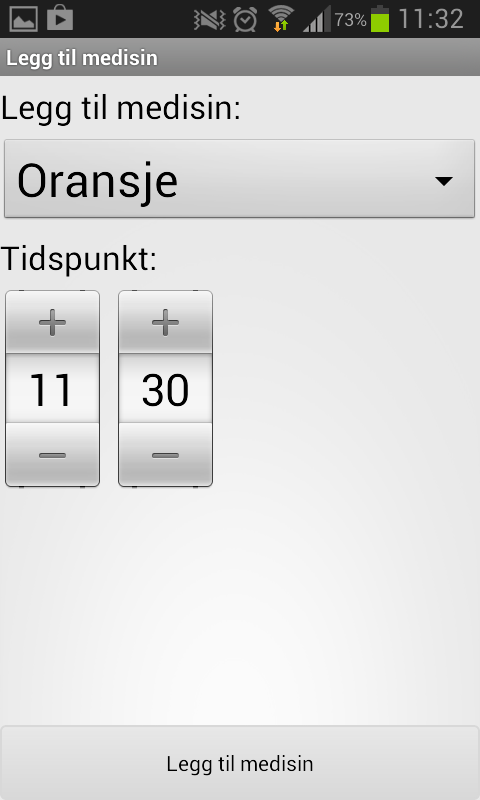
\includegraphics[width=0.20\paperwidth]{Pictures/new-screenshots/add-medicine-to-plan.png}
		\caption{Adding a medicine to a plan}
		\label{fig:add_medicine_to_plan}
	\end{minipage}
	\hspace{3cm}
		\begin{minipage}[t]{0.4\linewidth}
		\centering
			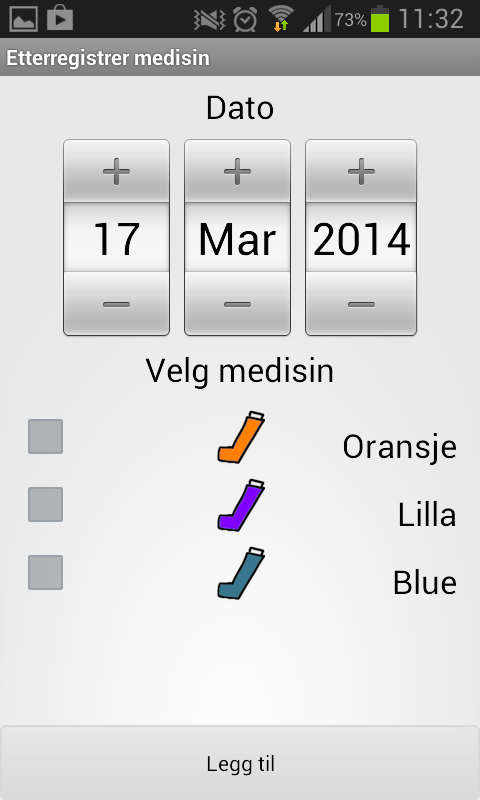
\includegraphics[width=0.20\paperwidth]{Pictures/new-screenshots/register-medicine-taken.png}
		\caption{Register a medicine that was taken without the help of \buddy{} or AsthmAPP}
		\label{fig:register_medicine_taken}
	\end{minipage}
	%NEW LINE
		\begin{minipage}[t]{0.4\linewidth}
		\centering
			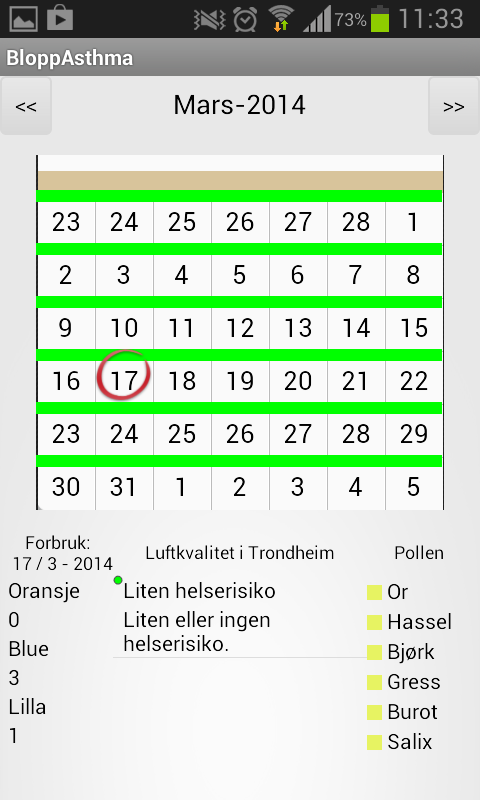
\includegraphics[width=0.20\paperwidth]{Pictures/new-screenshots/log.png}
		\caption{Medicine log}
		\label{fig:medicine-log}
	\end{minipage}
	\hspace{3cm}
		\begin{minipage}[t]{0.4\linewidth}
		\centering
			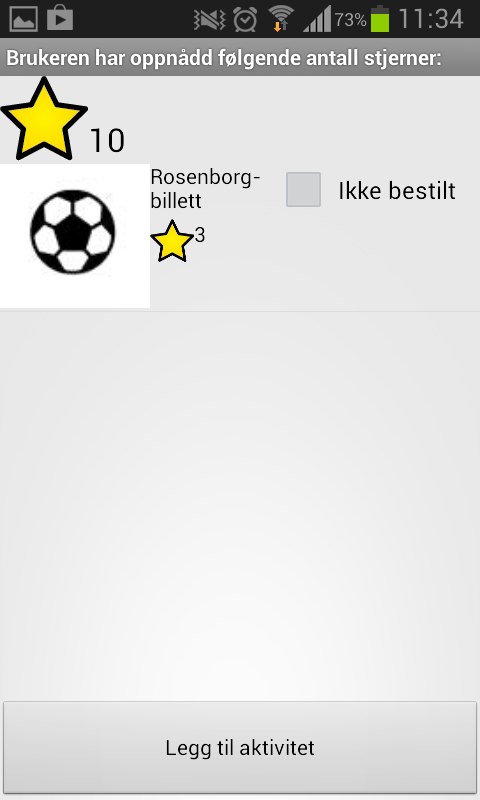
\includegraphics[width=0.20\paperwidth]{Pictures/new-screenshots/award.png}
		\caption{Overview of rewards a child can get}
		\label{fig:parent-awards}
	\end{minipage}
\end{figure}

\begin{figure}
	\begin{minipage}[t]{0.4\linewidth}
		\centering
			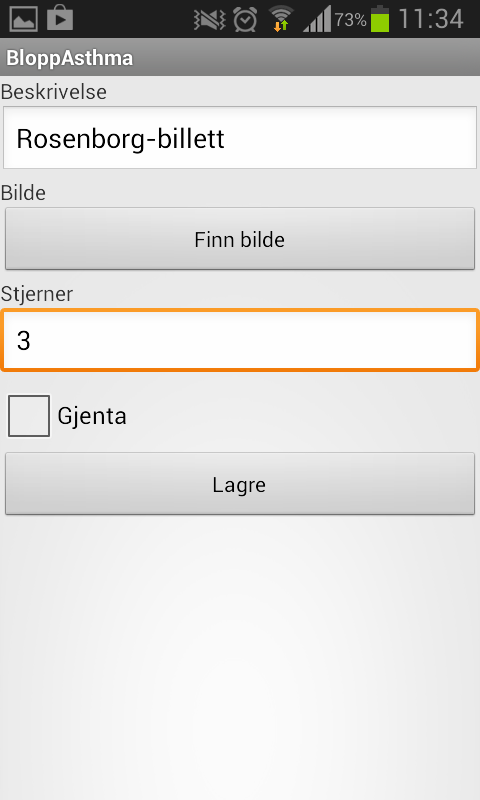
\includegraphics[width=0.20\paperwidth]{Pictures/new-screenshots/create-award.png}
		\caption{Creating a reward. Parents can either choose a reward from our standard image set, or they can take one from their gallery}
		\label{fig:parent-create-reward}
	\end{minipage}
	 \hspace{3cm}
	 \begin{minipage}[t]{0.4\linewidth}
		\centering
			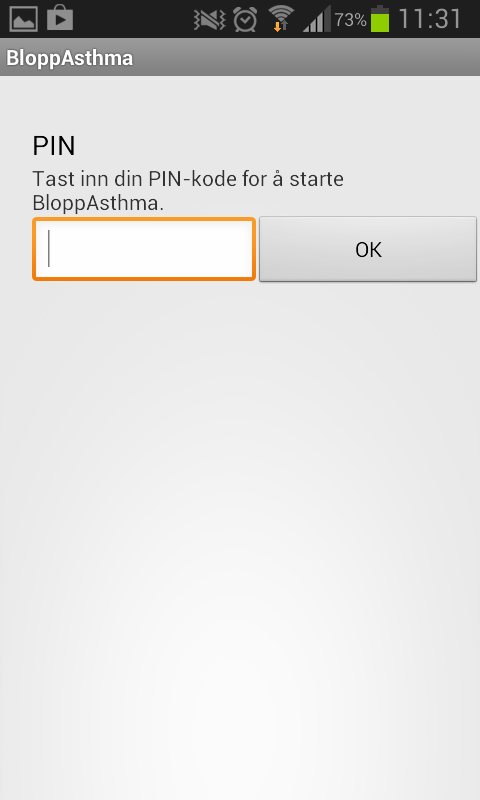
\includegraphics[width=0.20\paperwidth]{Pictures/new-screenshots/pin-challenge.png}
		\caption{In order to access the parent partition users have to complete a PIN-challenge}
		\label{fig:parent-pin}
	\end{minipage}
\end{figure}

\section{Parent Partition}
\label{sec:parentpartition}

\subsection{Menu}
\label{sec:description-menu}
Figure \ref{fig:parent_main_menu} shows the main menu of the parent partition. It has five options (Norwegian translation in paranthesis):
\begin{enumerate}
  \item Medicine Plan (\emph{Medisinplan})
  \item Register Medicine Afterwards (\emph{Etterregistrer medisin})
  \item Medicine Log (\emph{Medisinlogg})
  \item Rewards (\emph{Premier})
  \item Manual (\emph{Manual})
\end{enumerate} 

In order to access the parent partition the user is prompted with a PIN challenge. This was done in order to protect the child's medical data if a smart phone is lost or stolen. 

\subsection{Medicine plan}
\label{sec:description-medicine-plan}
Creating a medicine plan for asthma treatment is highly connected to the Traffic Light System explained in Appendix \ref{chp:traffic-light}.
Users can have three different plans, depending on which health state they are currently in. As we are targeting children, we can not assume that they are aware of which category they are currently in, and as a result, we let their parents control it. Figure \ref{fig:parent_medicine_plans} and \ref{fig:add_medicine_to_plan} shows the view in which one may change the medicine plan their child are currently on, in addition to setting alarms where appropriate. For instance, one may set an alarm at 07:00 AM, so that it reminds the user before it is time to leave for school. Changing the medicine plan is done by selecting the checkbox at the left side of the panel.  


\subsection{Register Treatment}
\label{sec:description-register-medicine}

If a child need to take their medicine, but do not have the possibilty to do the treatment with \ab{} or \app{} nearby, they can take their medicine and register the treatment later. This ensures that children are able to collect their stars even though they did not do their treatment with \ab{} or \app{} as their companion. Figure \ref{fig:register_medicine_taken} shows how this is solved in \app{}.  

\subsection{Medicine log}
\label{sec:description-medicine-log}
The \emph{Medicine log} can be used by parents to show how many times a child has taken his/her medicine. We assume that one of the main reasons for a child not taking his/her medicine is lack of communication between parents. A medicine log gives parents the ability to check and see whether the child has taken the necessary dose on any given day.


Figure \ref{fig:medicine-log} shows the calendar view of the application, which we will explain into details. The calendar module used is an open source component developed by Chris Goo, which we modified for our purposes. The cells show any given day of a month. In addition, there is a top bar which shows the health state (or health plan) of the child on the day selected below. At the bottom of the screen, there are three panels. The left panel shows which medicine has been taken on the selected day. The topbar of this panel indicates which day is selected. The middle panel shows the air quality in Trondheim\fnurl{Measured by NILU}{http://luftkvalitet.info/}. The right panel shows the pollen distribution of the 6 most common pollen types\fnurl{Measured by NAAF}{http://www.pollenvarslingen.no/}. The idea behind this is that asthma symptoms are often the same as allergy symptoms, and if parents are able to recognize a pattern between health state and pollen distribution, they may wish to take special precautions, such as no outdoor activity on a day with extreme amounts of pollen.    


\subsection{Manual}
\label{sec:description-manual}
The manual contains the same information as shown in Section \ref{sec:description-instructions}. The manual is added to both the parent partition and the child partition of the application. This is done because it is important for both the children and the parents to know how to use the medicine correctly. 


\subsection{Reward}
\label{sec:description-manage-rewards}
Figure \ref{fig:parent-awards} shows the list of possible rewards a child may receive. They are added by parents through \emph{Add reward}. The idea of having parents set their children's rewards is to specify rewards according to children's interest (see Section \ref{sec:gamificationinapp}). Figure \ref{fig:parent-create-reward} shows how one may add a reward. The user inserts a description, then either adds a photo or selects one out of our standard images. It is possible to set a reward on \emph{Repeat}, which will make the reward appear multiple times, each time with an increased cost.        
When the user press \emph{Save} (Lagre), the reward is added and the child has the possibility to select it. 
 
 
\section{Evaluation}
\label{sec:asthmappevaluation}
Chapter \ref{chp:gamification} gave an introduction to the term gamification, and how gamification should be used. We have developed a reward system that is highly based on parents' opinions, and thus, have some flaws that we will discuss further in the followin. 

First of all, children may become bored of the rewards if the rewards are not increasingly difficult to achieve, and have not increased in value. For instance, if a child is rewarded with a ticket to a football match for achieving 10 stars, and then receives a piece of gum if he/she achieves 20 stars, the child may lose interest and important motivation in order to complete his/her treatment. 

Secondly, the number of stars rewarded depends on the child's inferred health state (green state yields 1 star, orange state yields 3 stars and red state yields 5). This calculation of rewards leaves a possible exploit where children may pretend to be sicker than they are. In the long run, a child could fake being sicker than he/she actually is, just to achieve a reward more easily. This is a situation that \emph{could} occur, but we did not have the resources necessary to observe this pattern over time.

Thirdly, the gamification during the treatment, i.e. the animation on the phone, could become boring over time. 
The interactions are not varied, and it takes approximately 2 minutes to go complete a treatment. For expert users, who have had asthma for several years, it will become boring. Thus it should be noted that this is an application that probably would work best for young children in the early stage of their disease.      

In order to receive some expert opinion on our reward system, we asked a children psychologist, Nanna S\o nnichsen Kayed, who has expertise in reward systems for behavioral patterns among children, about the gamification parts of our system. 
She told us that letting parents choose when and what children should receive as rewards was good, but it has a downside. If the parents do not have an understanding as to how fast a child needs his/her reward, the child could easily loose interest. The amount of time necessary between each reward is higly individual. Preschoolers would need rewards almost every day, while a older children could manage with a reward twice a week. The part that is somewhat hard to understand here from a parent perspective, is that children needs to know they are rewarded for a treatment well done, and not necessarily something completely different. She proposed that if an application like this should be launched to an app store, a parental guide should follow along, as parents often do not understand this principle.

Furthermore, there has to be a balance between the rewards a child receives, and the work they are actually doing. For instance, a child cannot receive a bike after completing three treatments. Parents also have a materialistic mindset, i.e. rewards have to be something material. Kayed implies otherwise. Letting children choose a dinner, which TV program to watch at nighttime, or even being allowed to eat their breakfast under the table could be just as effective and fun as giving them tangible rewards. In order to equalize rewards across families, she concluded that parents already do this in other ``domains'', like allowance.   



